\chapter{Leaping Rainbow}

The aim of the game is to get the ball into the bowl. The player controls the ball using the mouse. When the game starts, the bowl bounces from the left side of the screen to the right side, leaving behind a rainbow trail. The player must control the ball to pass only along the arc. If it does not touch the rainbow - the game starts over.

\begin{figure}[H]
   \centering
   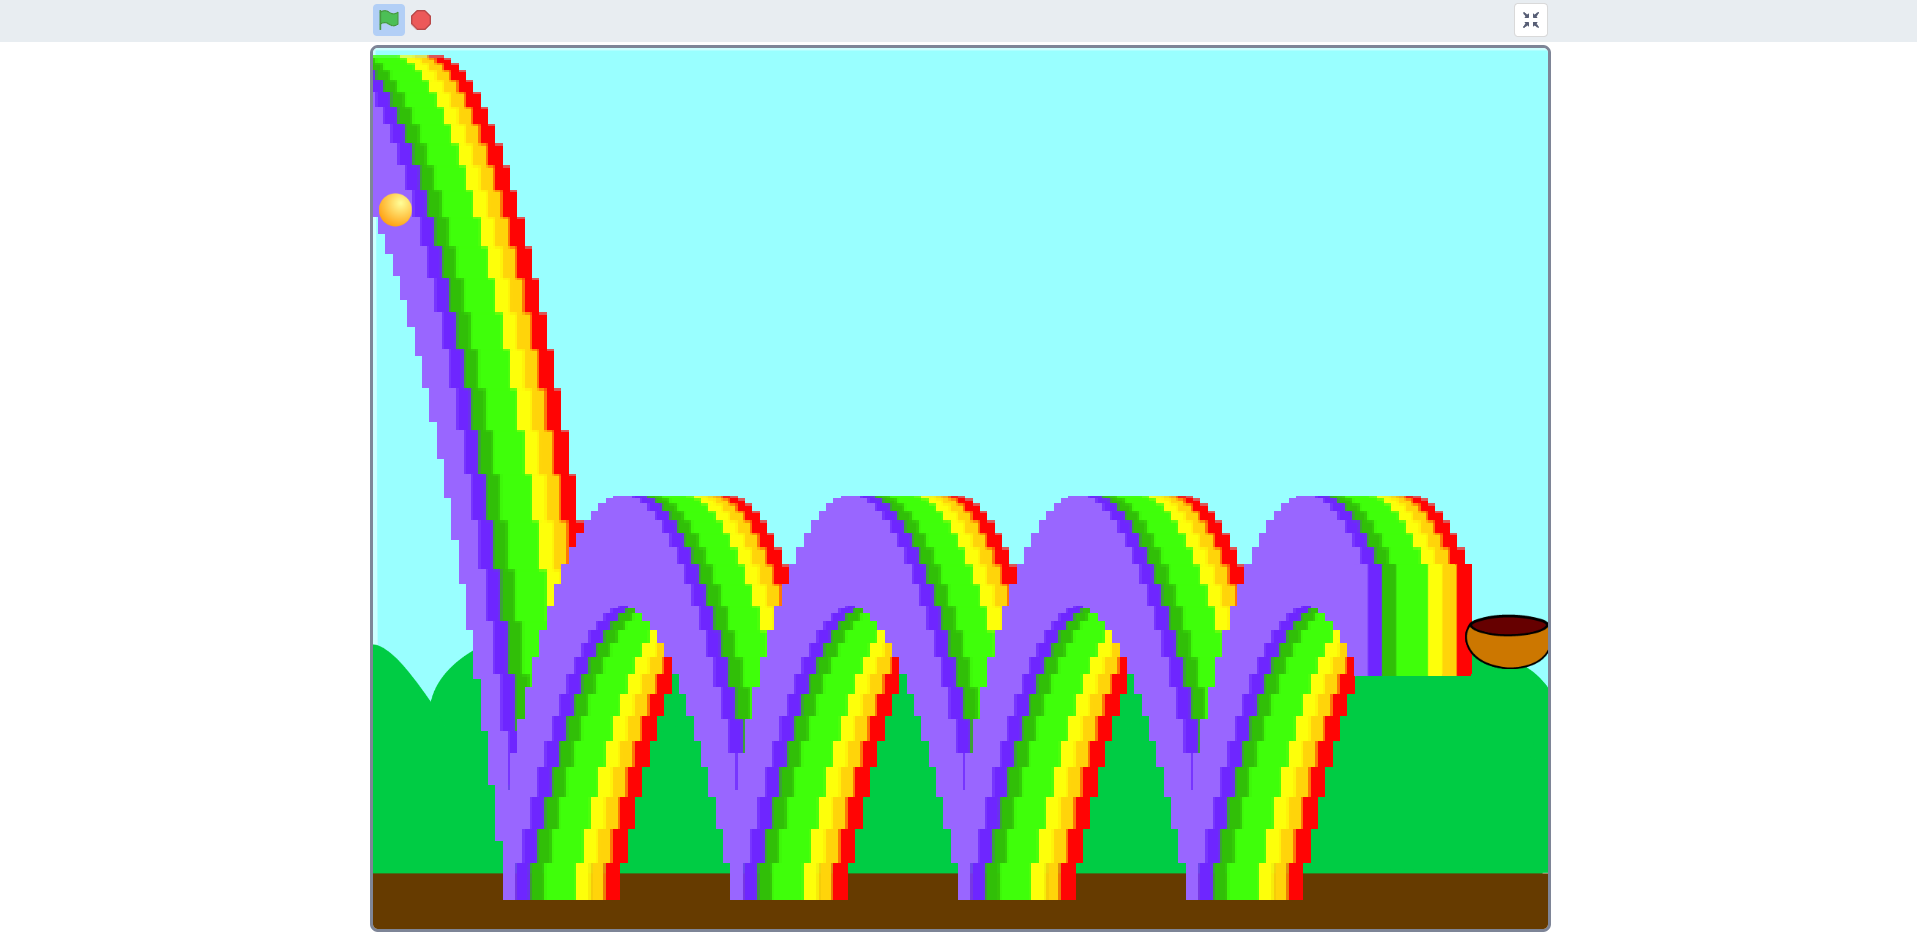
\includegraphics[width=1.0\linewidth,height=0.5\linewidth]{fig070001.png}
   \caption{Leaping Rainbow}
\label{fig070001}
\end{figure}

\section{Adding Background and Characters}
The first step of the game is to add a suitable background and characters. The characteristic of the background is that there should be a brown band at the bottom, which will serve as a reference point. If the background to be selected is not there, it can also be added using the drawing tools.

The main character is not needed in this game. For that, he should be deleted. The characters bowl and ball are among the ready-made characters in Scratch. The rainbow character must be drawn (Fig. \ref{fig070002}).

\begin{figure}[H]
   \centering
   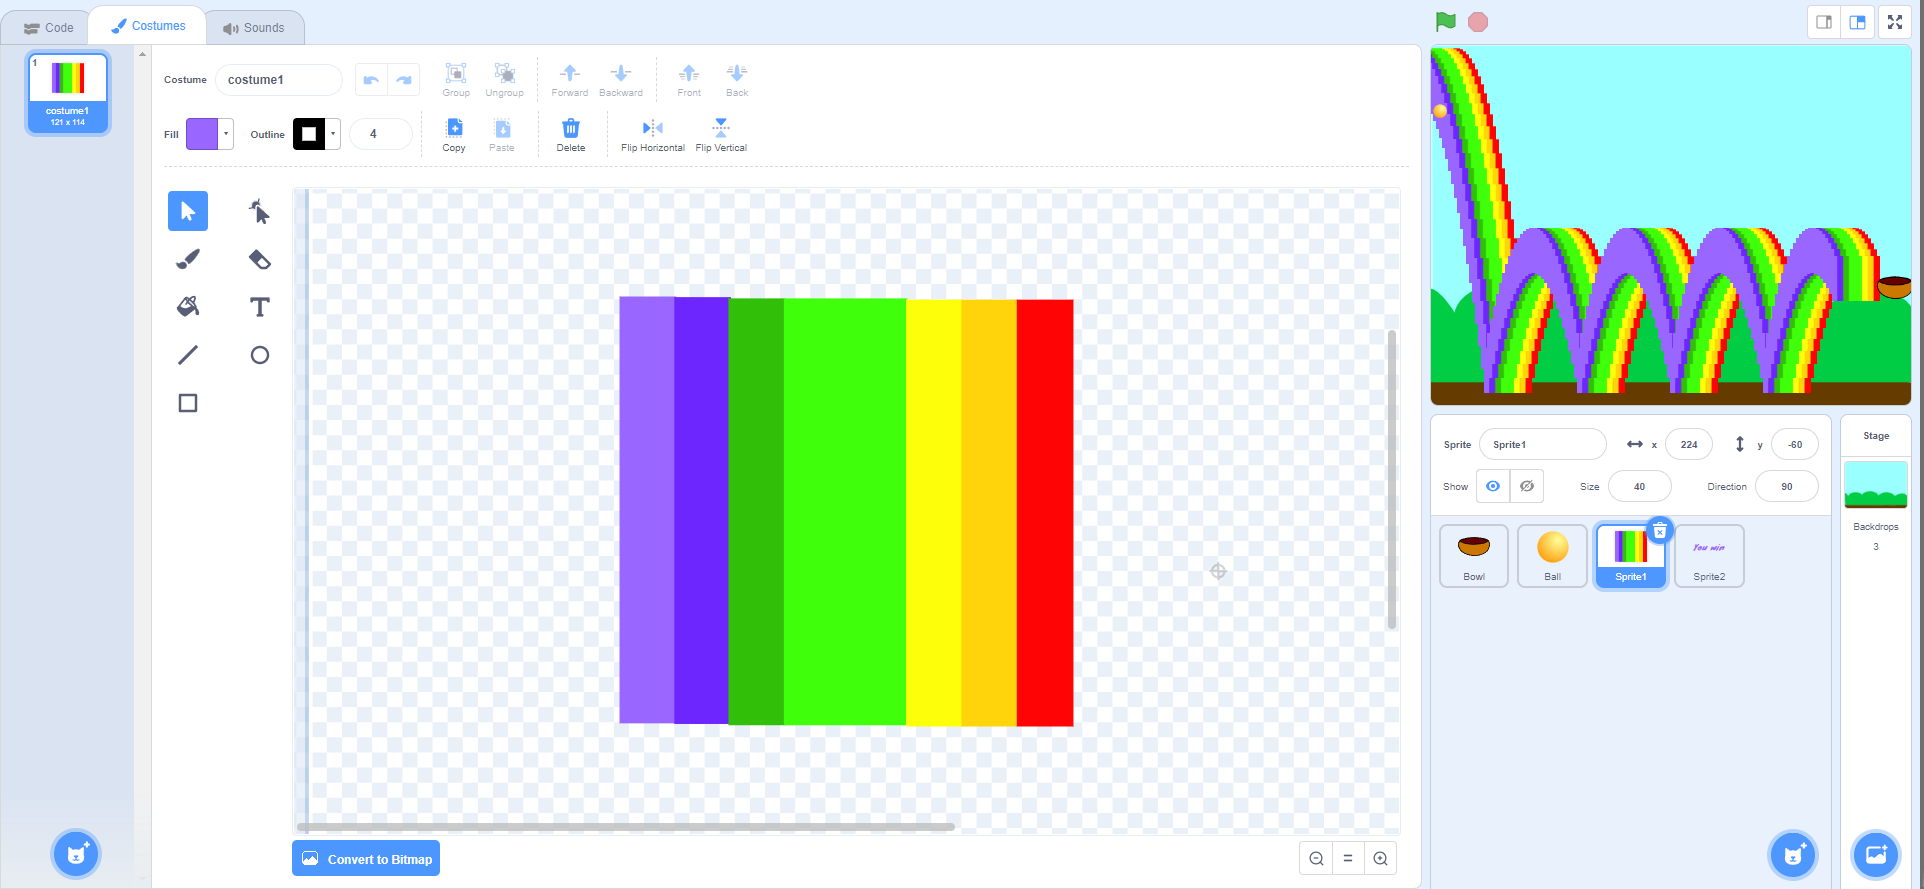
\includegraphics[width=1.0\linewidth,height=0.5\linewidth]{fig070002.png}
   \caption{Adding the character arc}
\label{fig070002}
\end{figure}

One more character needs to be drawn. This inscription will appear when the ball touches the bowl, i.e., the player successfully goes through the entire arc.

\begin{figure}[H]
   \centering
   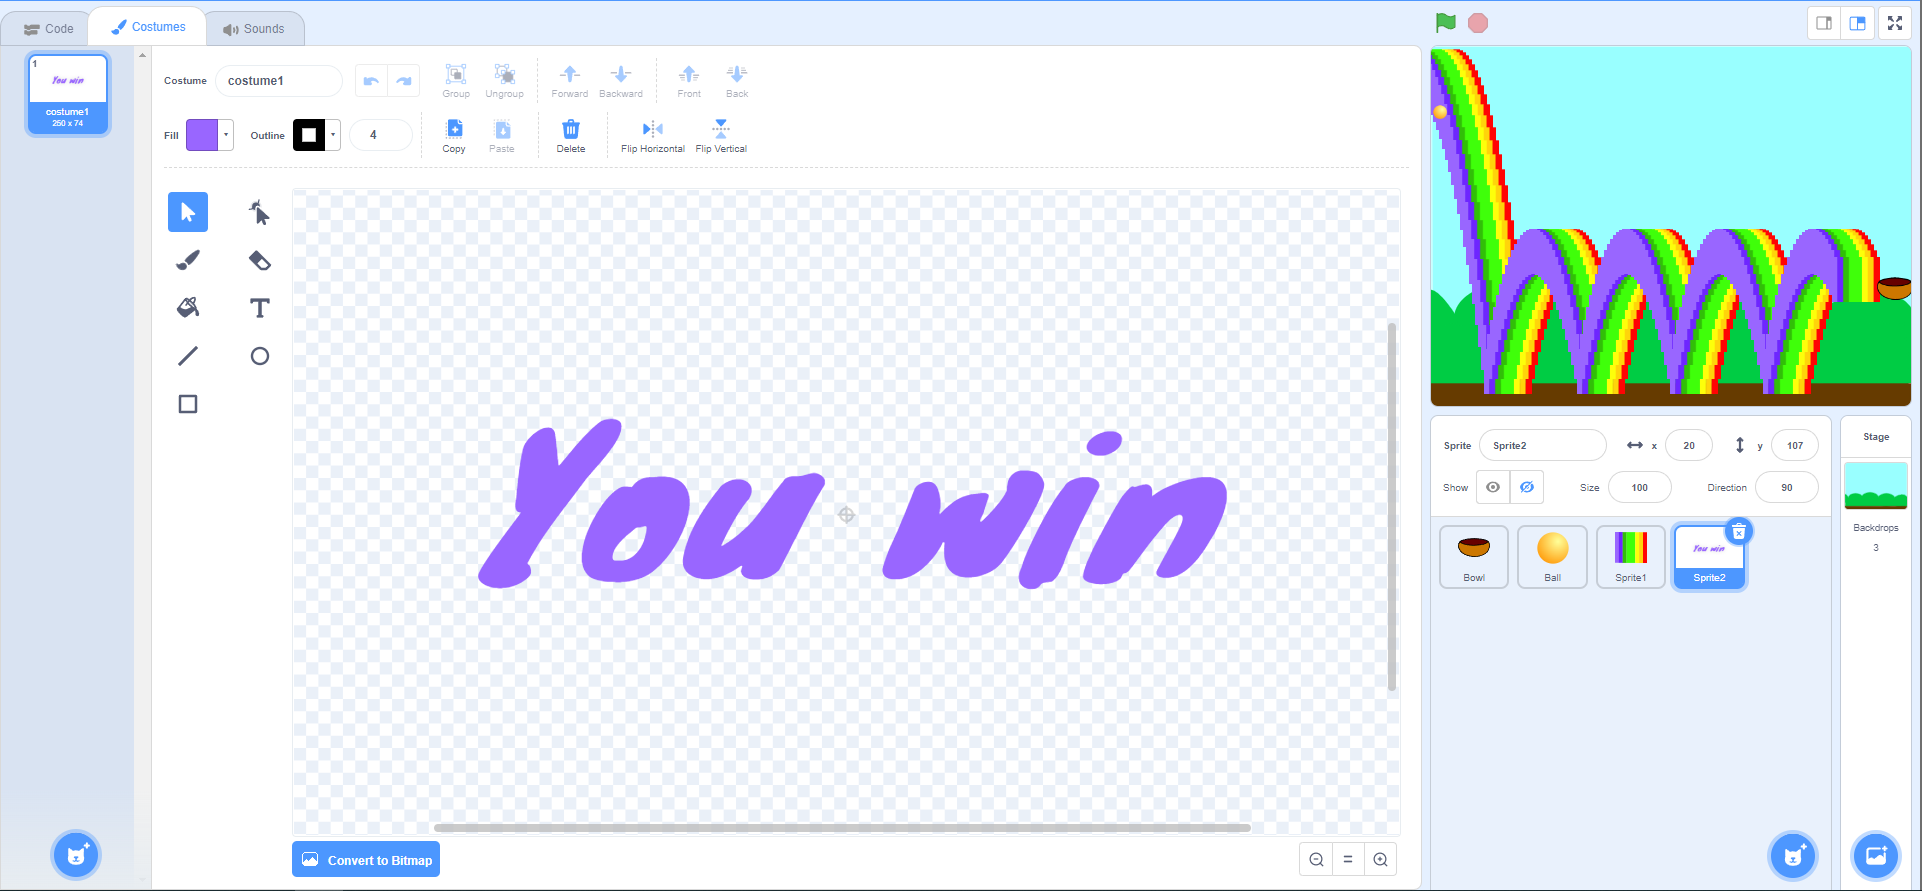
\includegraphics[width=1.0\linewidth,height=0.5\linewidth]{fig070003.png}
   \caption{Adding the character to end the game}
\label{fig070003}
\end{figure}

\section{Programming the Bowl}
The first instructions to be constructed are those for the bowl. Her goal is to go from the left side of the screen to the right by bouncing. The algorithm to be built for the bounce effect requires the creation of a variable. This variable will contain the value by which the y-coordinate will be changed. Until the bowl touches the brown border, the variable will decrement by 1. When it touches the border, it will take a value of 15.

When the game starts, the cup position should be on the left side of the screen. This means that the value of the x-coordinate should be -199 and that of the Y-coordinate 148. The initial value of the "velocity" variable should be equal to 0. The size of the character should be changed to be smaller.

\begin{figure}[H]
   \centering
   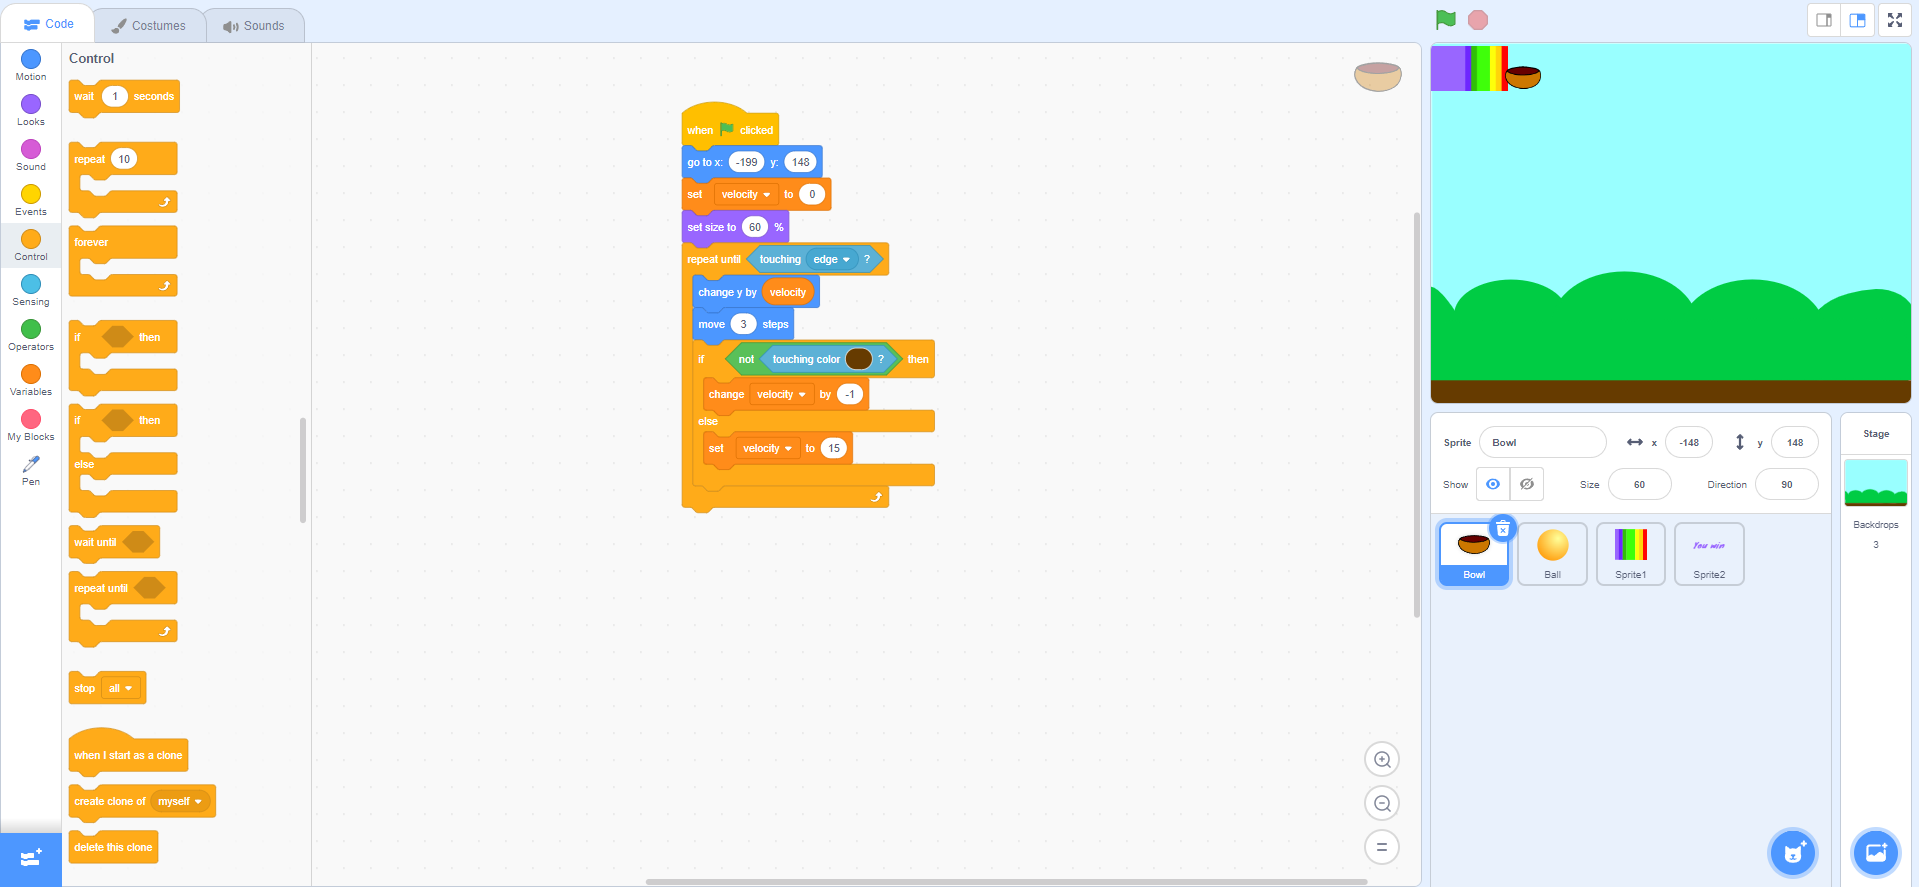
\includegraphics[width=1.0\linewidth,height=0.5\linewidth]{fig070004.png}
   \caption{Position of Hero Cup}
\label{fig070004}
\end{figure}

The movement of the bowl must be programmed. This movement must be repeated, meaning that a loop must be added with a goal "until the character touches an edge". This means that the character will move until it touches the right part of the screen. In addition to moving the character with the 3-step movement instruction, it must also change its y coordinate with the value of the "velocity" variable.

An if/else should be added to check if the character touches the brown border. If it is not touching it, then the variable must be decreased to move the character down. If it touches the border - the variable must have the value 15. To check that the brown color is not touched, a negation instruction must be added, located in the green group. The color check is in the light blue group. To find the exact color, use the eyedropper tool by placing it on the brown color. By instructions, the movement algorithm looks like this:

\begin{figure}[H]
   \centering
   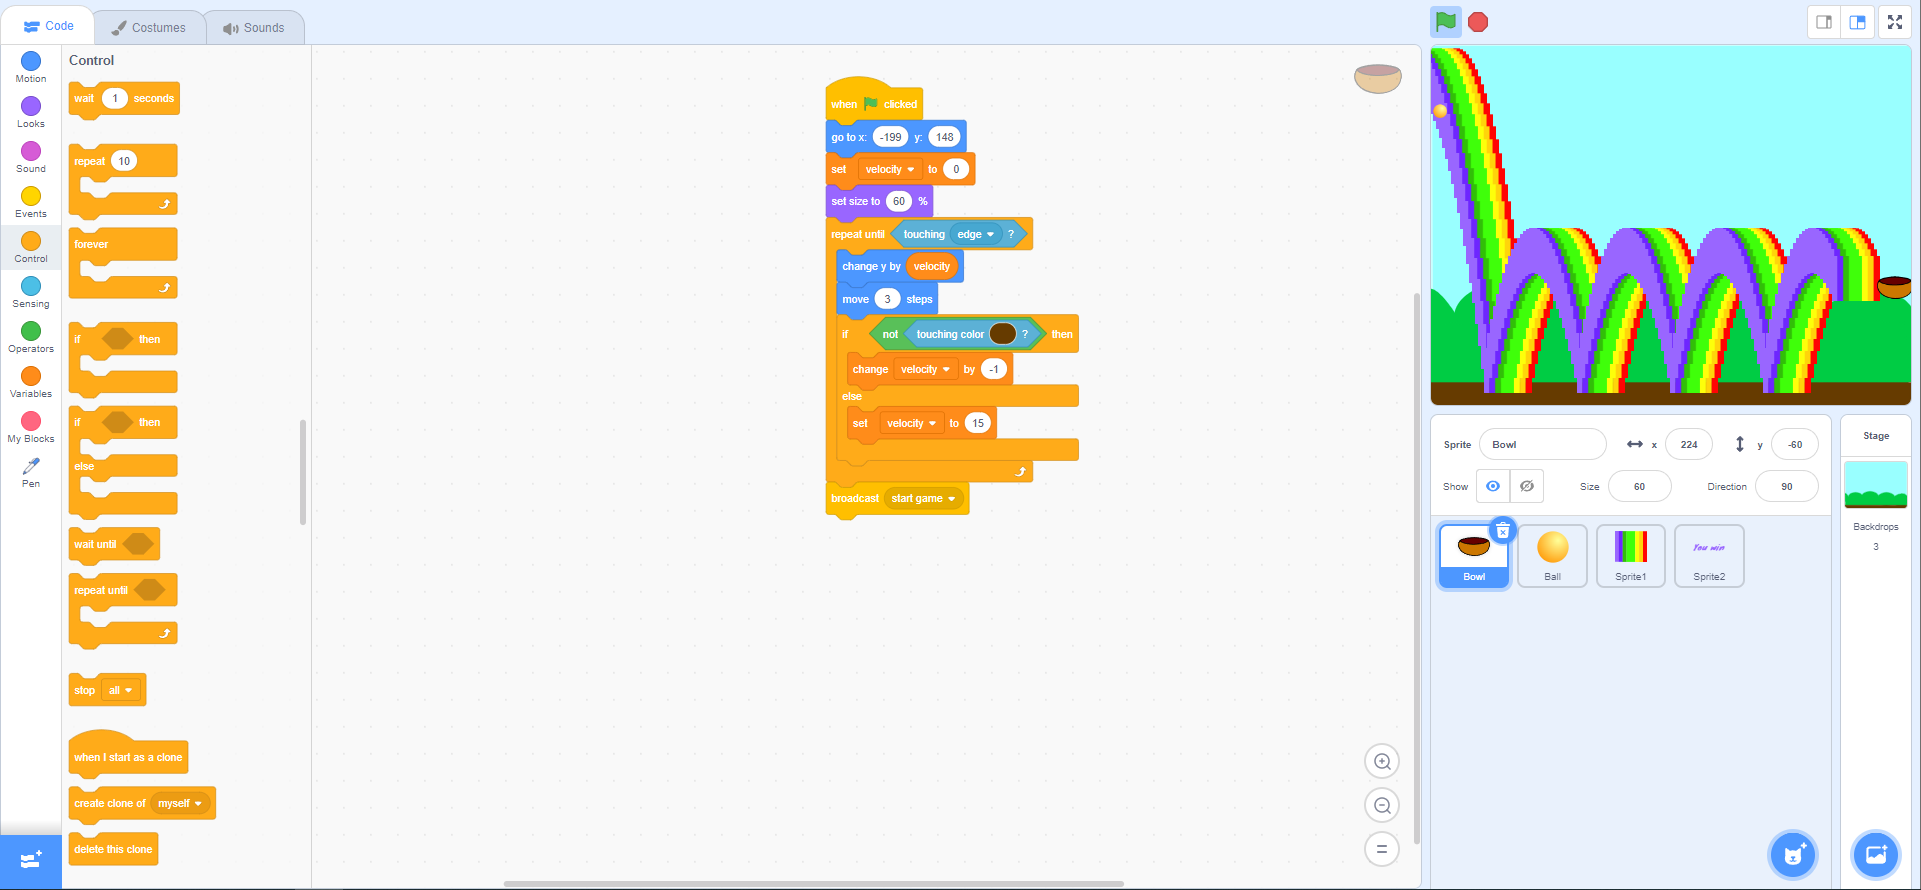
\includegraphics[width=1.0\linewidth,height=0.5\linewidth]{fig070005.png}
   \caption{Movement of hero cup}
\label{fig070005}
\end{figure}

After reaching his goal, the character must send a "start game" message. Only then can the game begin. Instructions for sending messages are located in the yellow instructions group.

\begin{figure}[H]
   \centering
   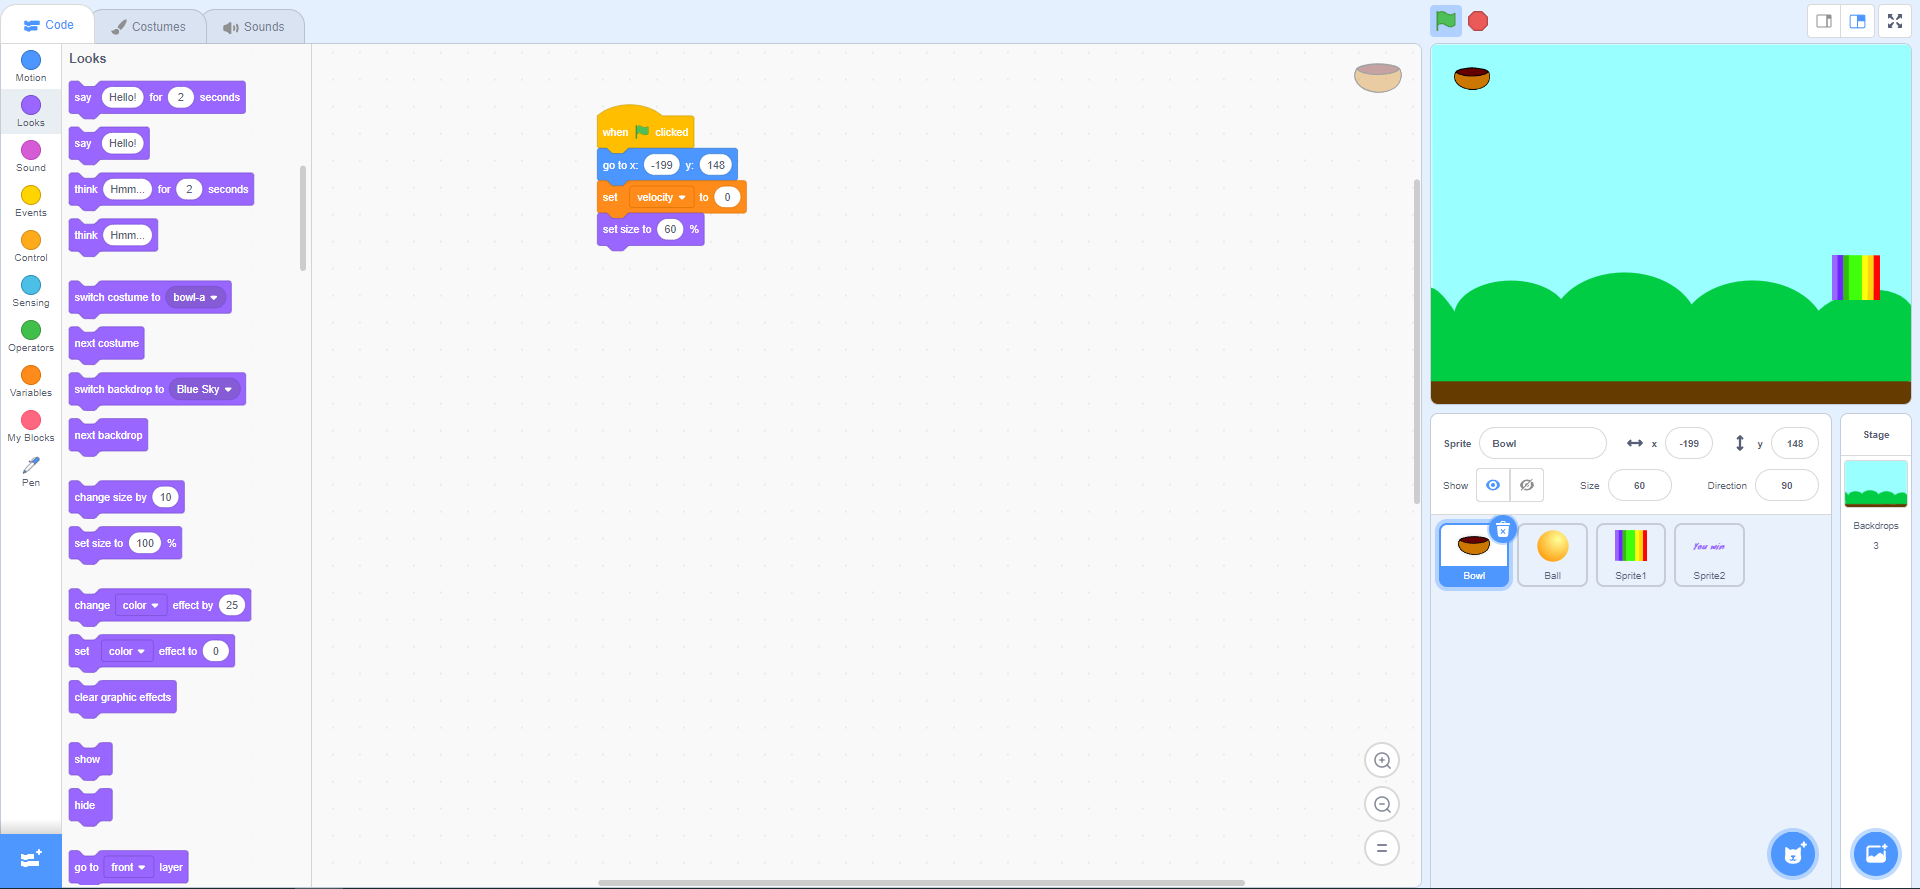
\includegraphics[width=1.0\linewidth,height=0.5\linewidth]{fig070006.png}
   \caption{The Hero Cup Code}
\label{fig070006}
\end{figure}

When the game starts, it is noticed that the character goes from one part of the screen to the other, jumping.

\section{Programming the Rainbow}
To program this character to leave traces, a new group of instructions must be added - A pen.

\begin{figure}[H]
   \centering
   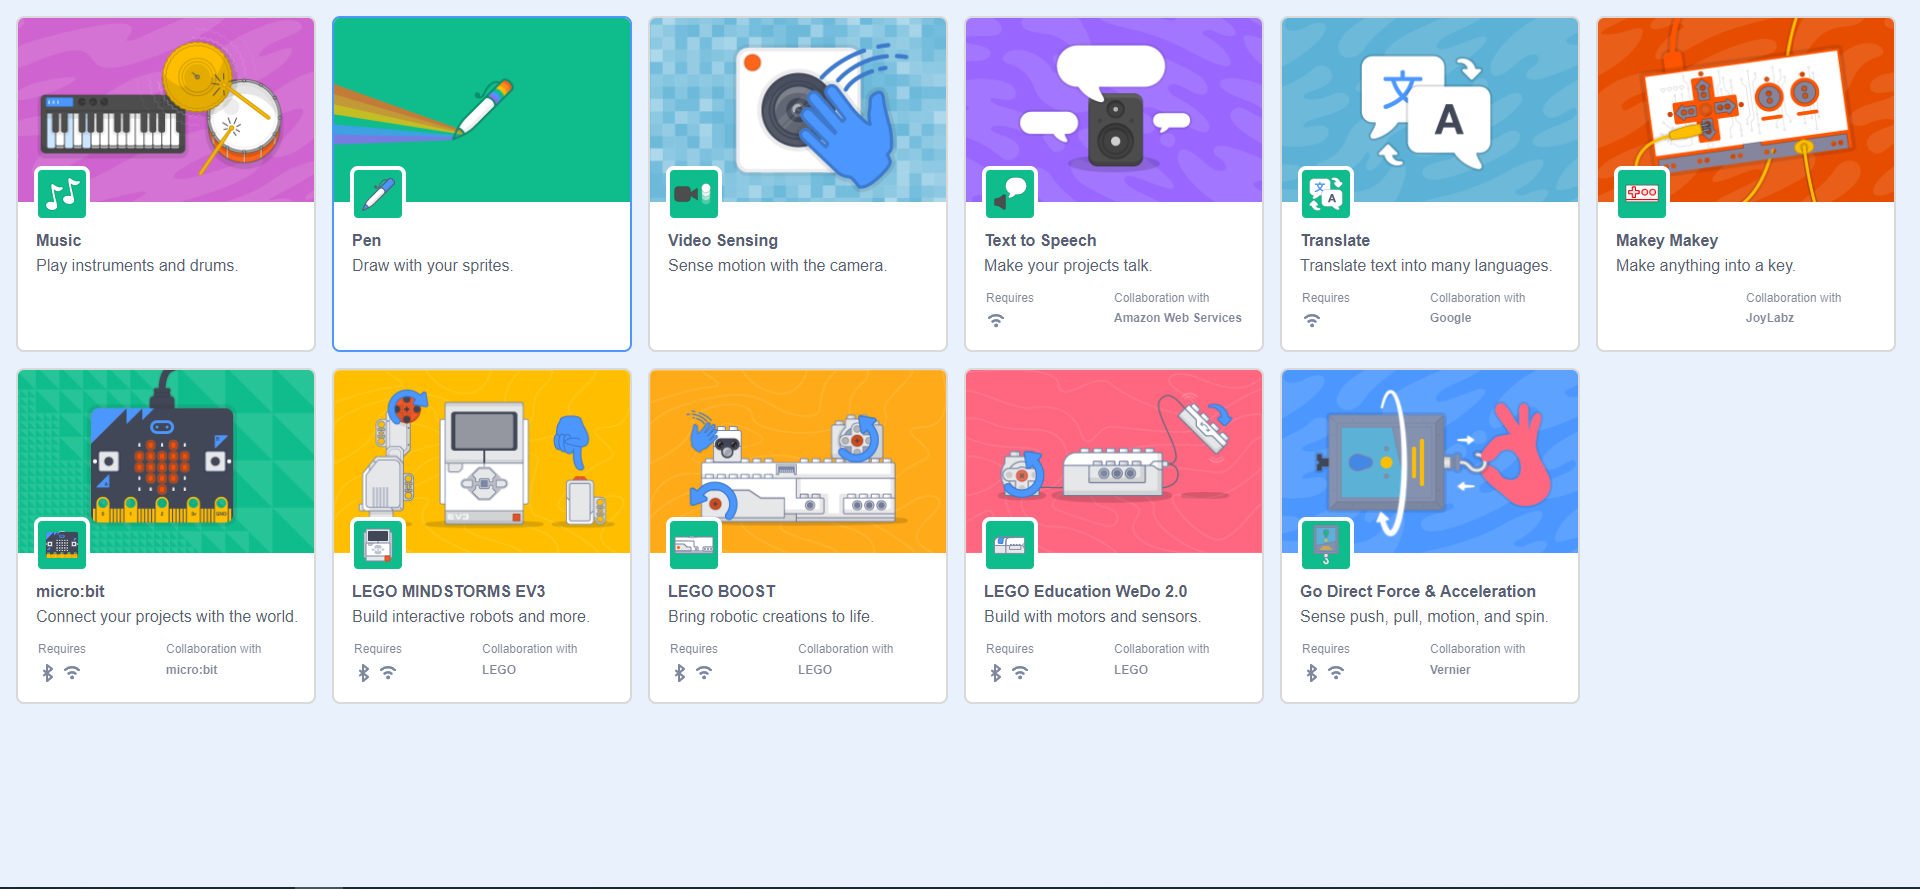
\includegraphics[width=1.0\linewidth,height=0.5\linewidth]{fig070007.png}
   \caption{New group of Pen instructions}
\label{fig070007}
\end{figure}

Based on how the character is drawn, it should be reduced. This can be done without instructions but by changing the Size property.

\begin{figure}[H]
   \centering
   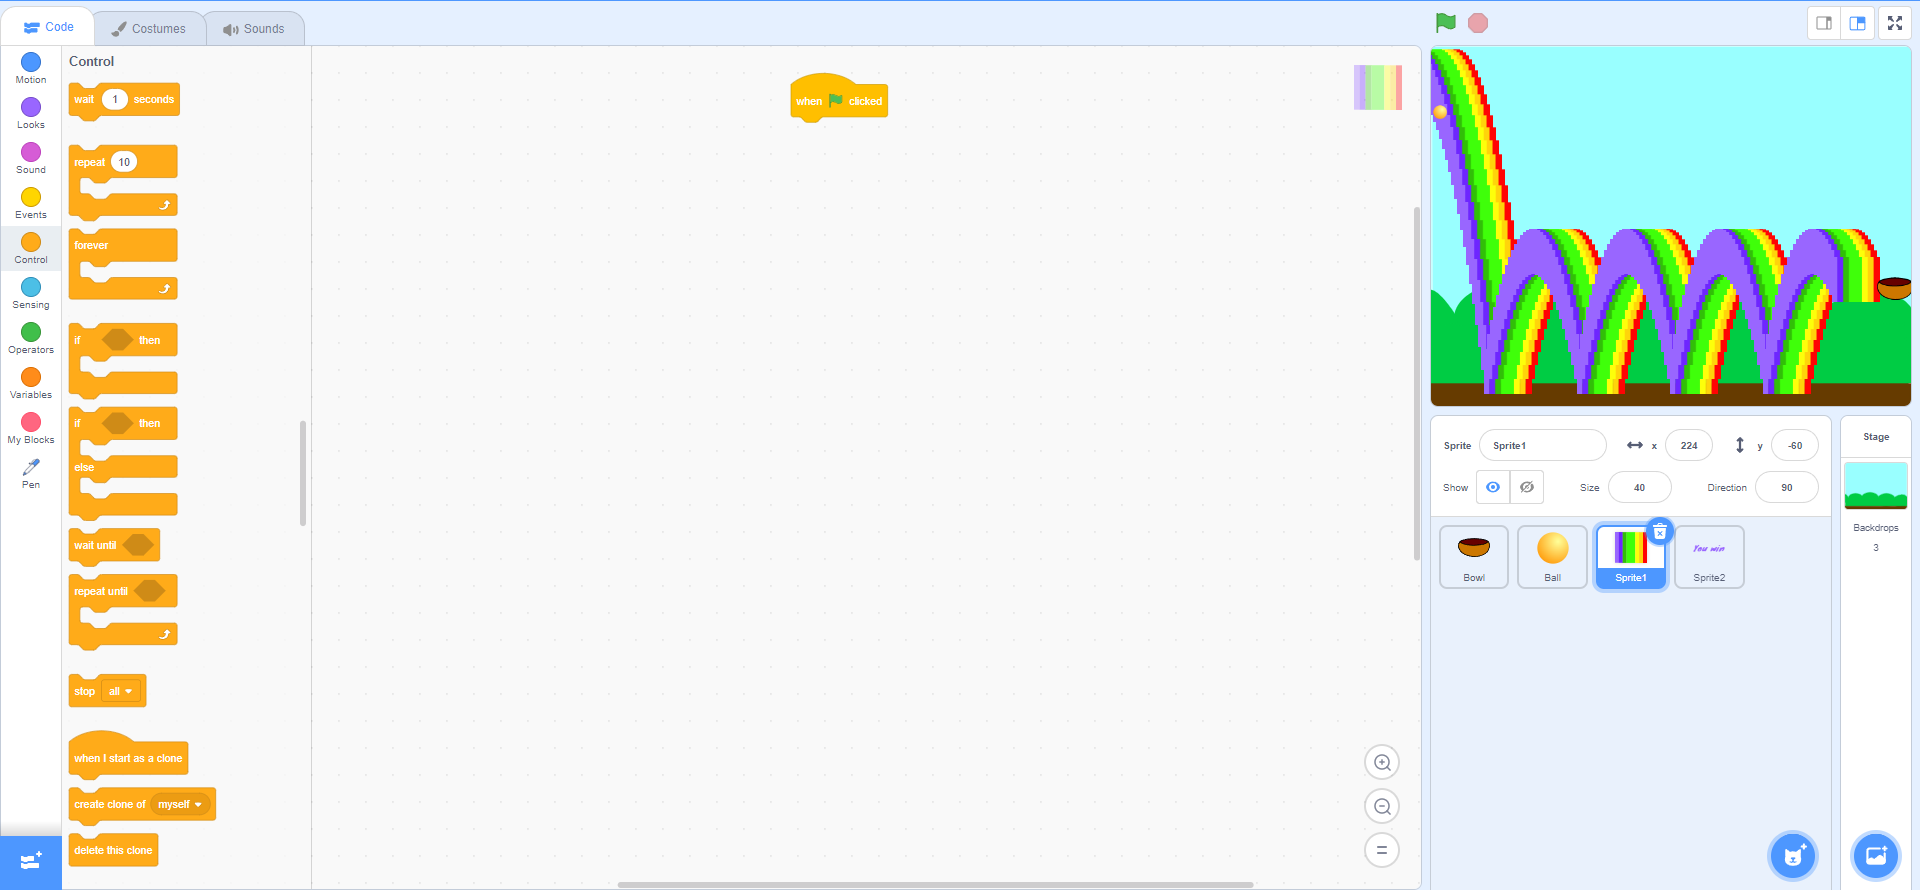
\includegraphics[width=1.0\linewidth,height=0.5\linewidth]{fig070008.png}
   \caption{Change the Size property}
\label{fig070008}
\end{figure}

This character's instructions are to follow the cup character and leave tracks. At the beginning of the game, everything drawn must be erased. This is done using the "erase all" instruction in the newly added instruction group. In addition to following the movement of the bowl character, the rainbow must follow its direction. This is done using the instruction from the blue "point in direction" group. An instruction from the light blue group, which is "backdrop of Stage", should be used to indicate exactly which direction to follow. First, the second value of the "Stage" of the character name is changed. Then the type is also changed, which should be "direction".

\begin{figure}[H]
   \centering
   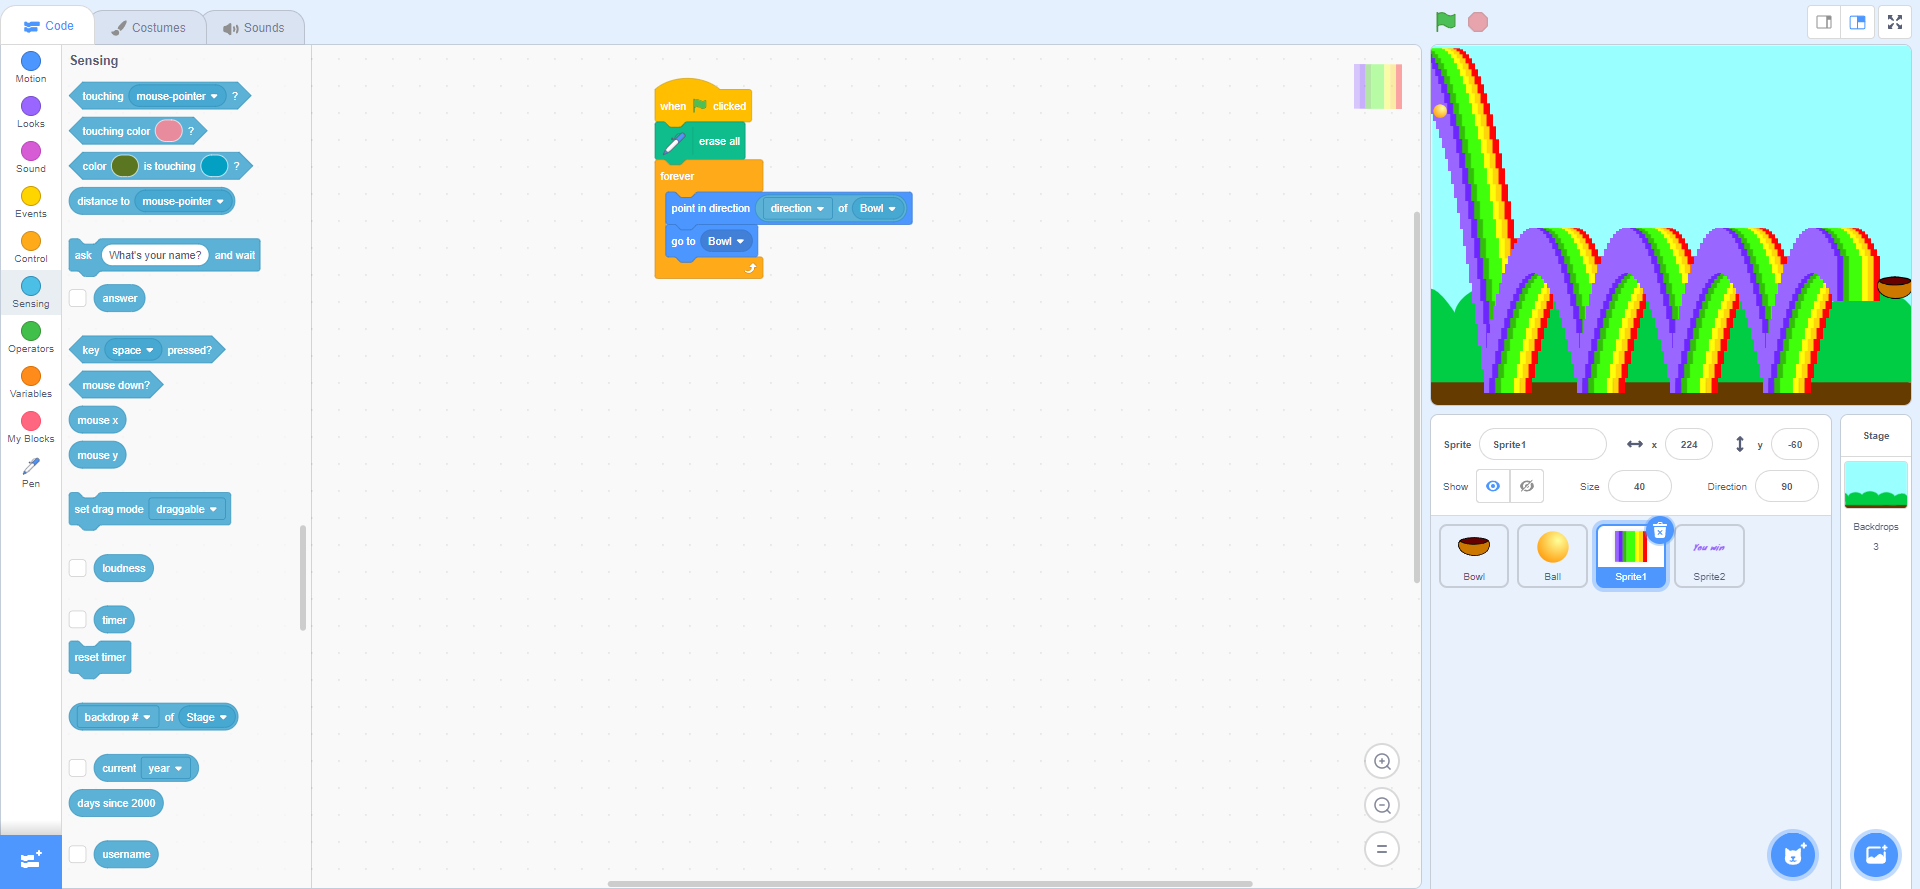
\includegraphics[width=1.0\linewidth,height=0.5\linewidth]{fig070009.png}
   \caption{Movement of the character arc}
\label{fig070009}
\end{figure}

If you start the program, you will notice that the rainbow character only follows the cup character. The "stamp" instruction found in the new group must be used to leave a mark.

\begin{figure}[H]
   \centering
   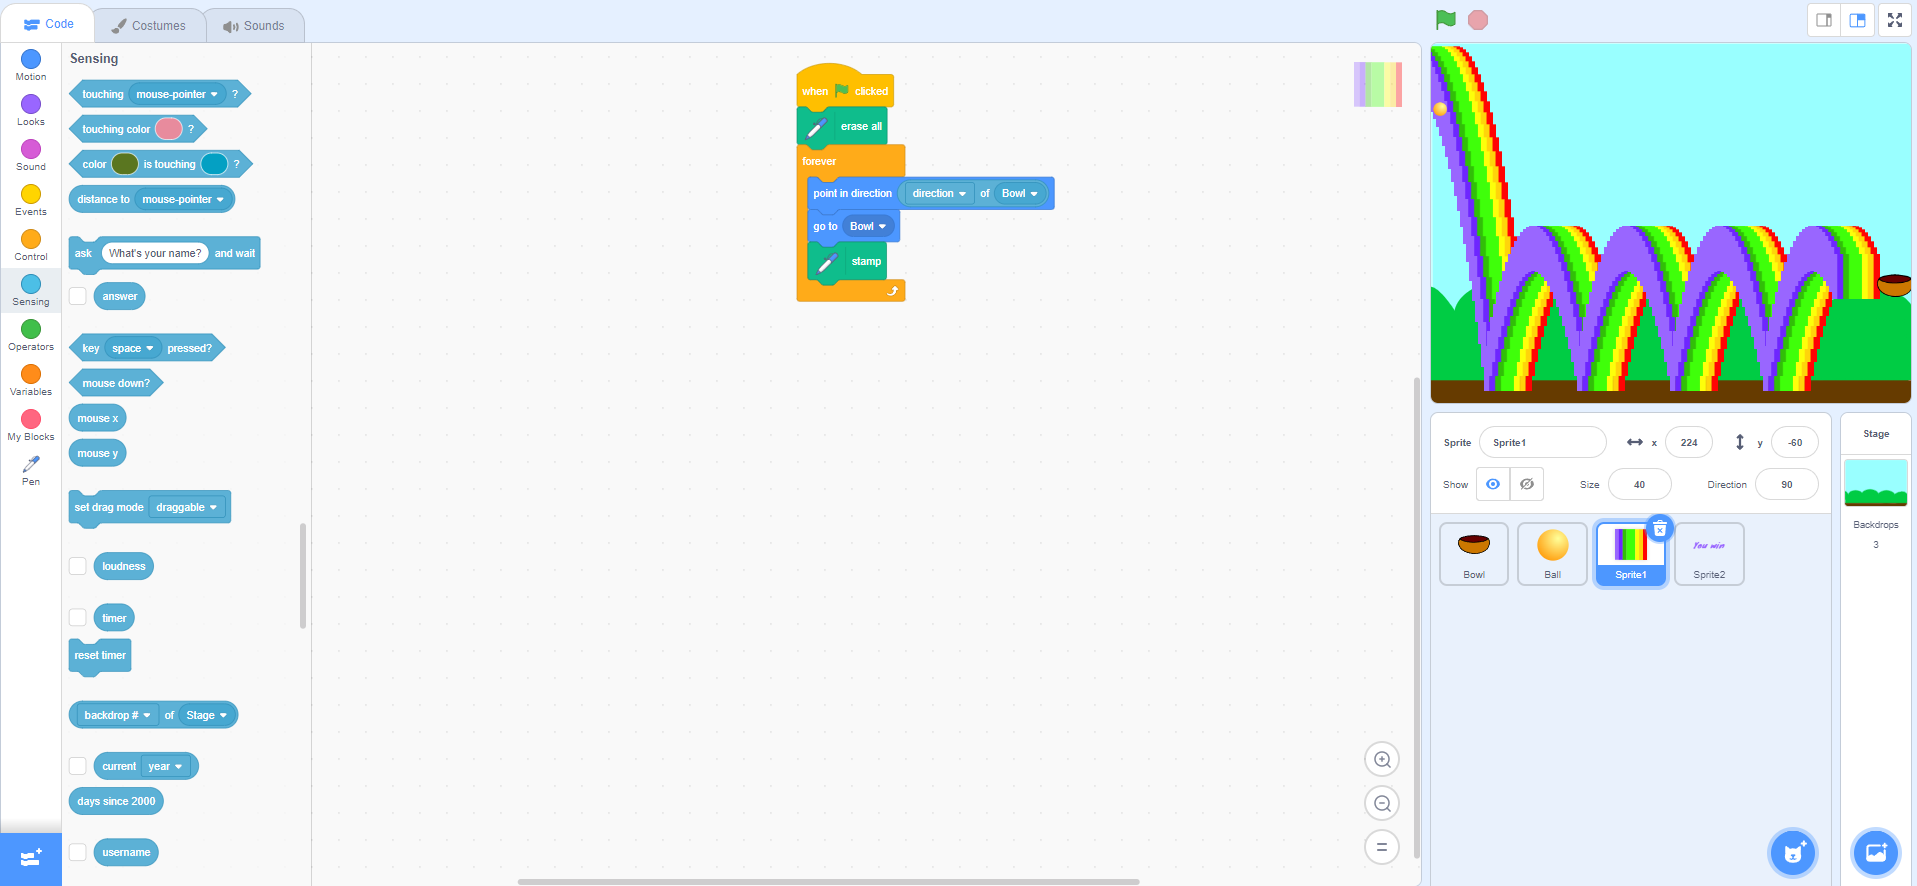
\includegraphics[width=1.0\linewidth,height=0.5\linewidth]{fig070010.png}
   \caption{All character code arc}
\label{fig070010}
\end{figure}

\section{Programming the Ball}
The dimensions of the ball must be such that it can pass through the entire rainbow touching the purple (or outermost) color. These can be changed by changing the value of the Size property.

\begin{figure}[H]
   \centering
   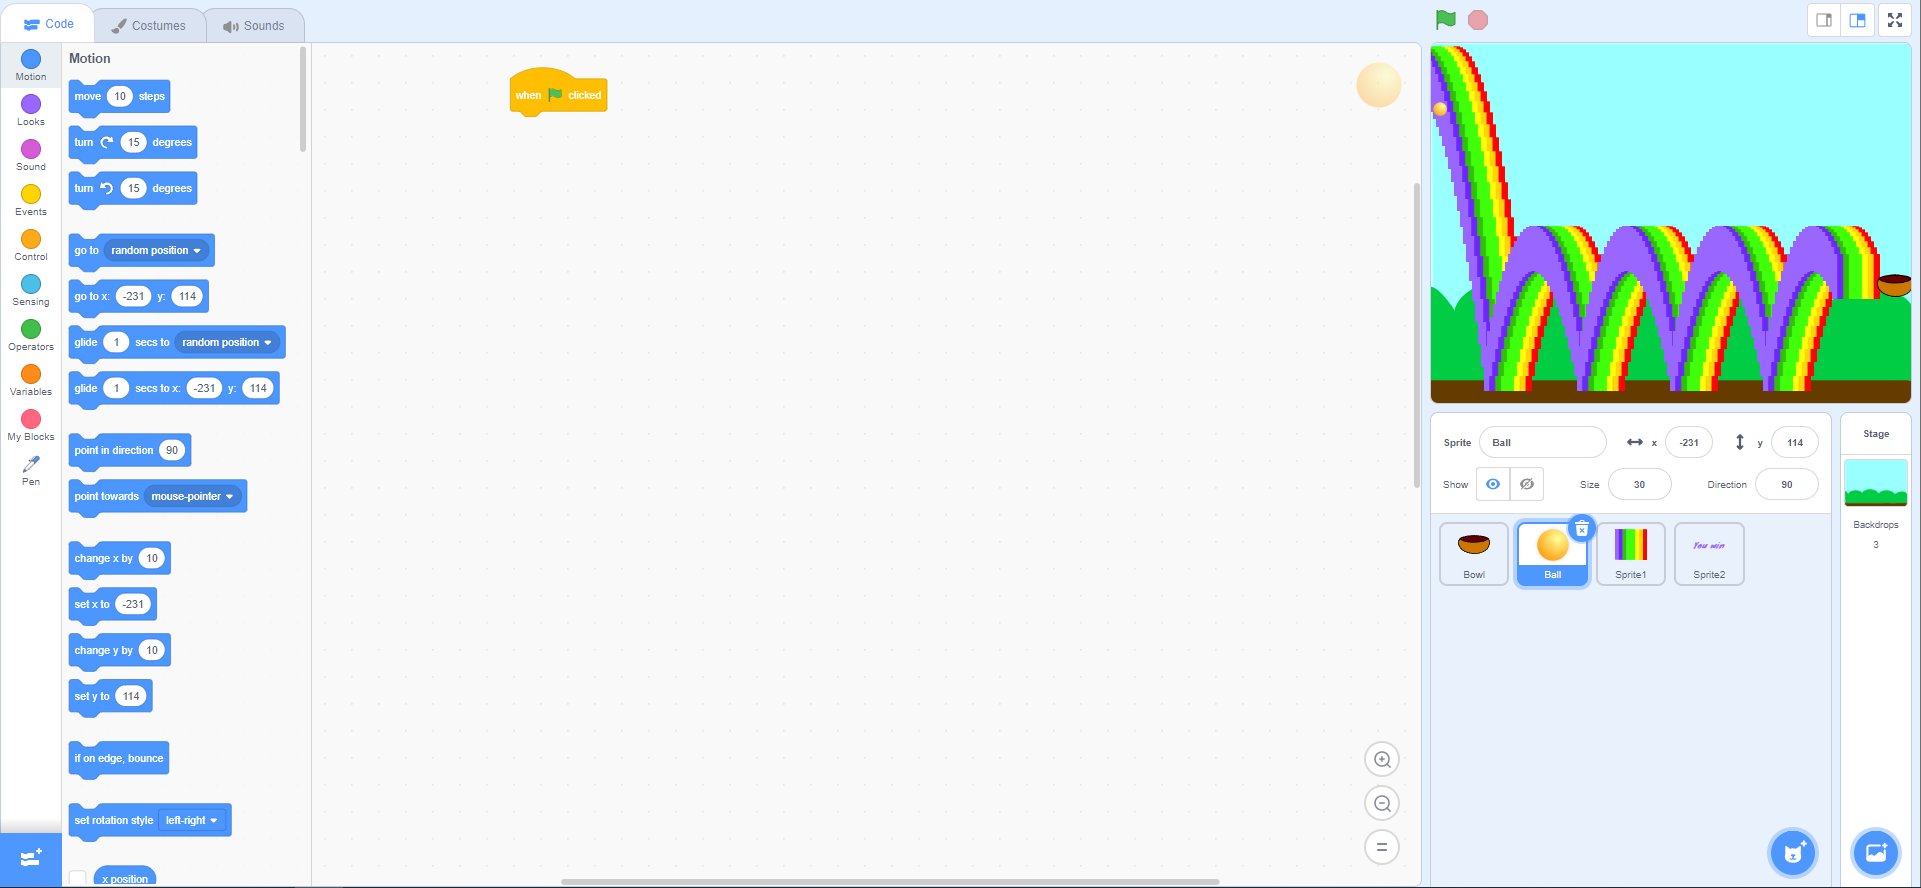
\includegraphics[width=1.0\linewidth,height=0.5\linewidth]{fig070011.png}
   \caption{Hero Ball Size}
\label{fig070011}
\end{figure}

The ball should appear when the bowl reaches the end of the screen. By instructions, this means when the character gets the "start game" message, then it appears. When the green flag is pressed, it should be hidden. When displayed, a slight animation can be made to move it to a position with coordinates for x=-231 and y=114.

\begin{figure}[H]
   \centering
   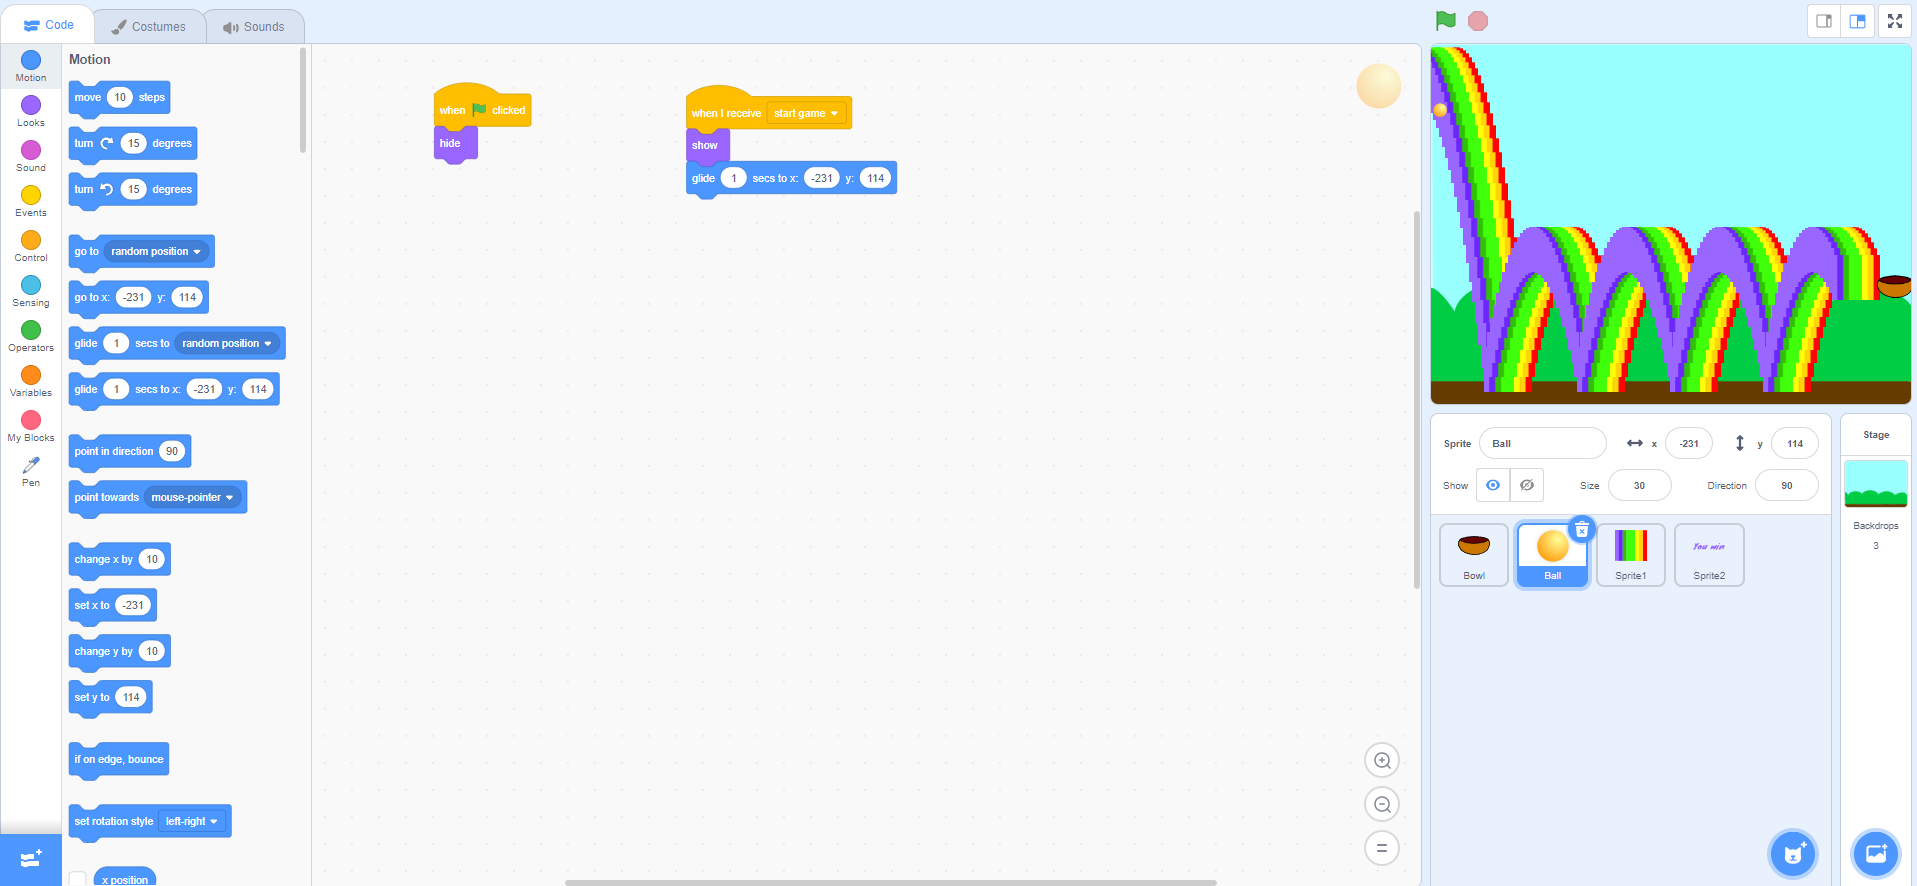
\includegraphics[width=1.0\linewidth,height=0.5\linewidth]{fig070012.png}
   \caption{Starting position of the ball character}
\label{fig070012}
\end{figure}

The character should start moving when pressed. It moves as it touches the outermost color - in this case, purple. Again, a loop with a goal should be used. The goal should be "until you stop touching the color purple". The statements outside the loop will be executed when the condition is false. In this case, it means moving to the starting position when the character does not touch the arc.

The movement instruction should be - follow the mouse. This instruction is in the blue group and goes to the mouse pointer. If the character needs to move slower, this is done by adding the wait instruction from the orange group.

\begin{figure}[H]
   \centering
   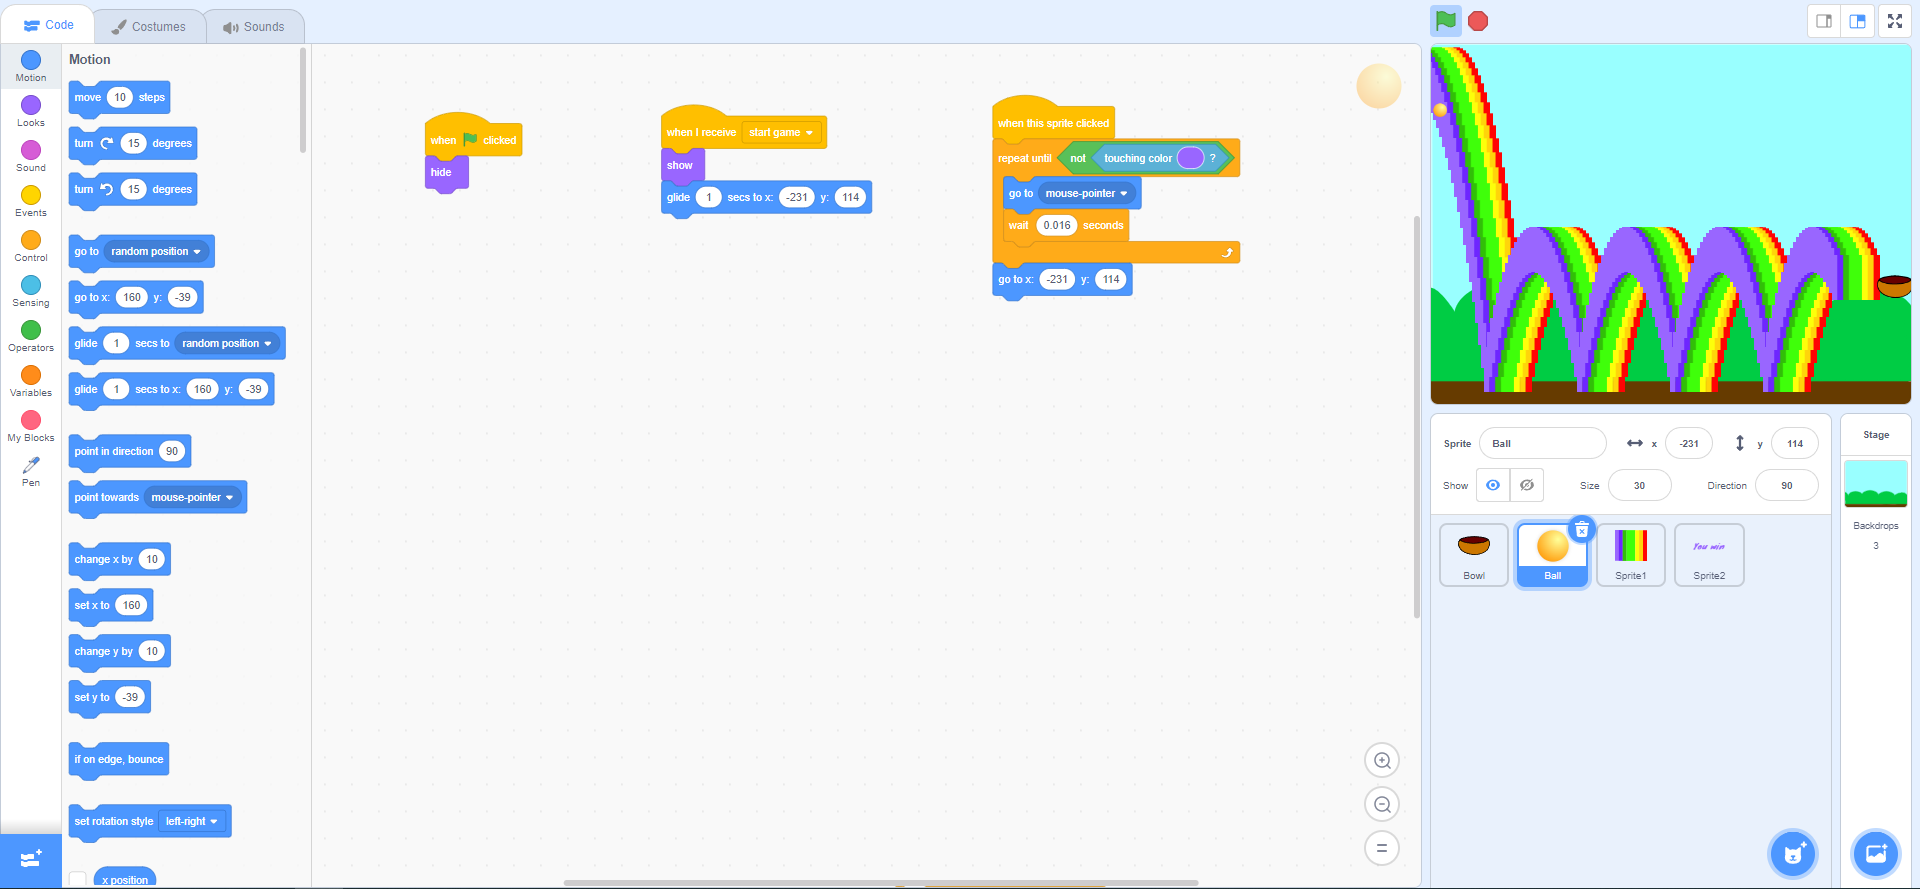
\includegraphics[width=1.0\linewidth,height=0.5\linewidth]{fig070013.png}
   \caption{Movement of character ball}
\label{fig070013}
\end{figure}

The last thing to do is check if the character has reached the end of the arc. If it is, then it will send a message to the character that is captioned to appear, and the game will end. At the end of the arc is the arc hero. Then checking whether to end the game is easy - as the ball touched the rainbow. If it is - it sends a message and ends the game. If not, the game continues.

\begin{figure}[H]
   \centering
   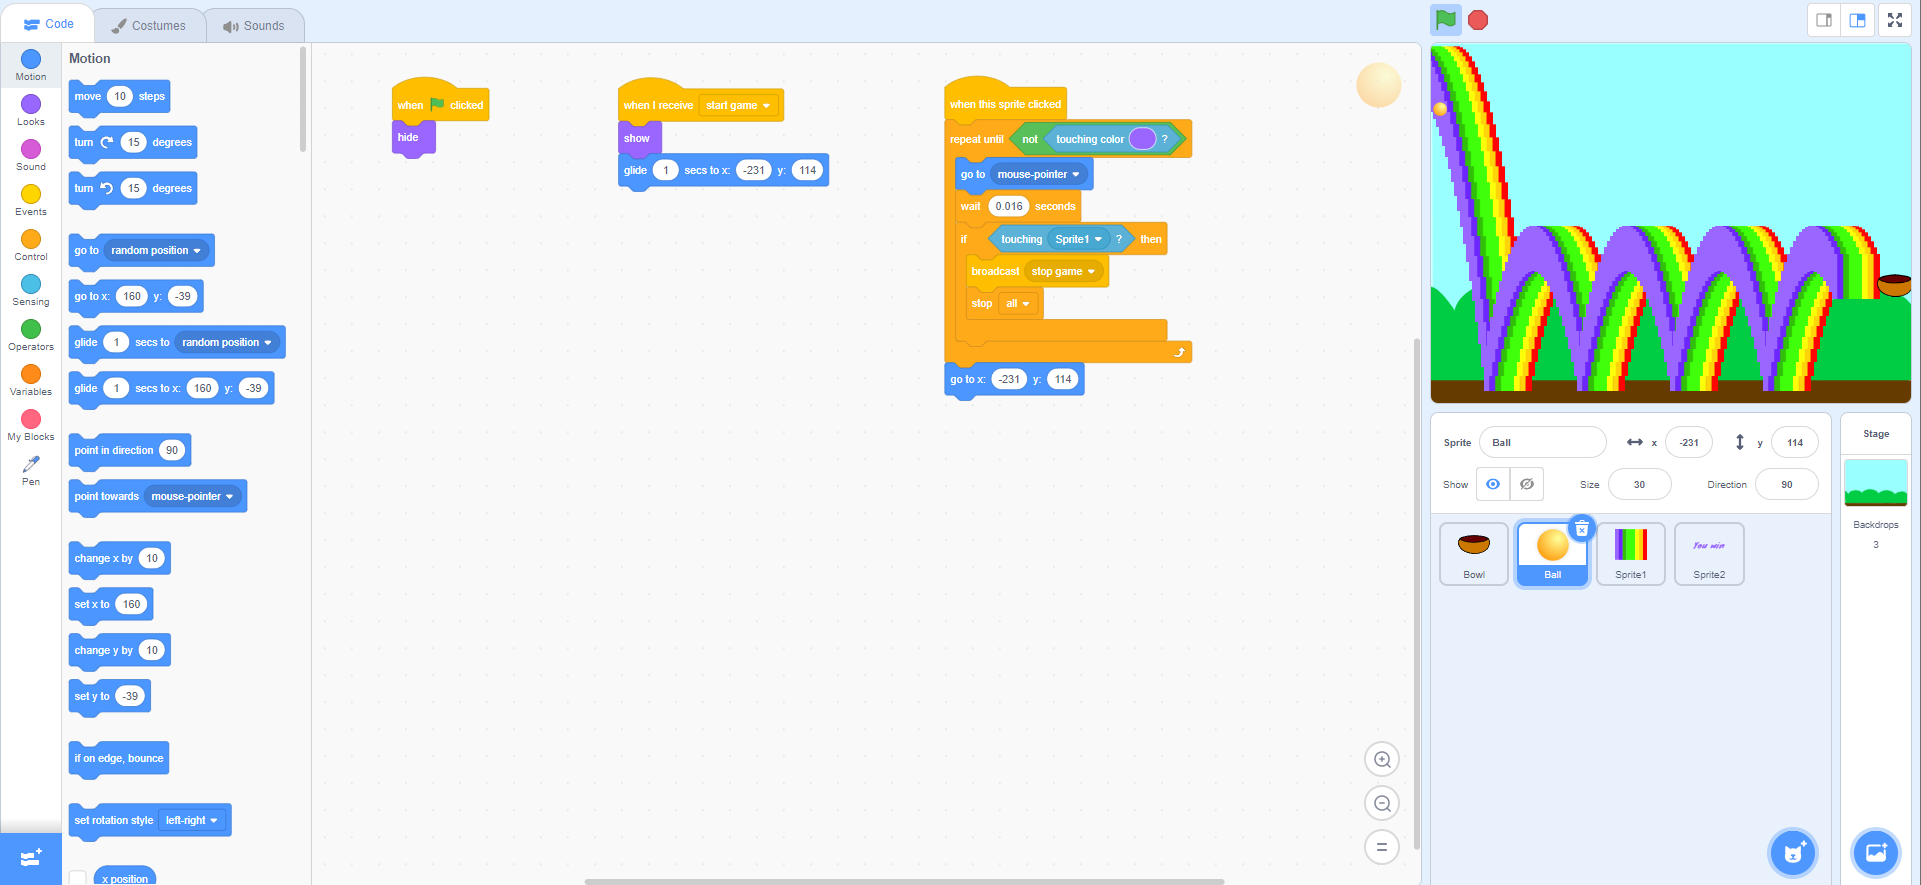
\includegraphics[width=1.0\linewidth,height=0.5\linewidth]{fig070014.png}
   \caption{The Orb Hero Code}
\label{fig070014}
\end{figure}

\section{End Game}
The character at the end of the game must be hidden at the beginning. It appears when the ball sends an end-of-game message.

\begin{figure}[H]
   \centering
   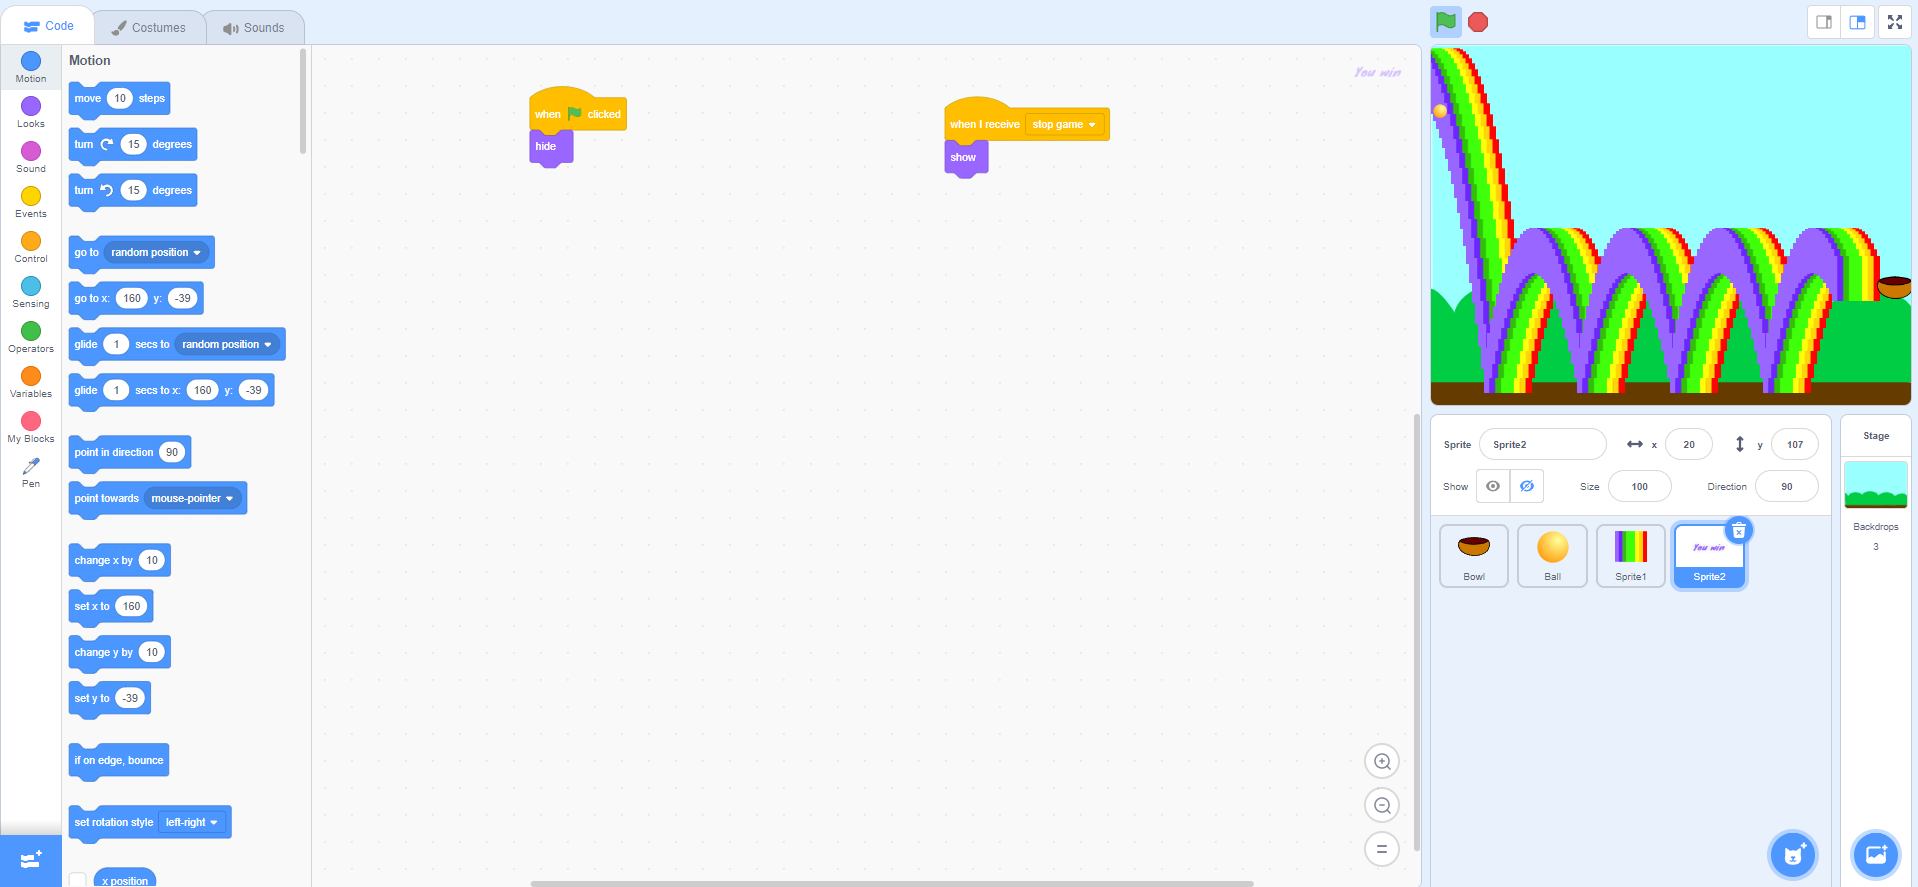
\includegraphics[width=1.0\linewidth,height=0.5\linewidth]{fig070015.png}
   \caption{Hero Code Caption}
\label{fig070015}
\end{figure}
